\documentclass{article}
\usepackage{amsmath}
\usepackage{amssymb}
\usepackage{fancyhdr}
\usepackage[utf8]{inputenc}
\usepackage{tcolorbox}
\usepackage[left=1in, right=1in, top=1.5in, bottom=1in]{geometry}
\usepackage{tikz}
\usepackage{enumerate}
\usepackage{enumitem}
\usepackage{pgfplots}
\usepackage{ragged2e}
\usepackage{tabularx}
\usepackage{array}
\usepackage{mdframed}

\pagestyle{fancy}
\fancyhf{} % Clear all header and footer fields
\fancyhead[L]{Your Name} % Left header with name
\fancyhead[R]{September 18th 2025} % Right header with date
\renewcommand{\headrulewidth}{0.4pt} % Horizontal line below the header

\newmdtheoremenv{theo}{Theorem}

\begin{document}

% Main title
\begin{center}
    \Large \textbf{Math 115E Activity WIP} \\
    \vspace{0.2cm}
    \normalsize Chapter 4 Section 1 \\
    \normalsize Average Rate of Change
\end{center}

\begin{mdframed}
\textbf{Definition.} 
\textit
    {
    The Average Rate of Change of a function $f(x)$ between two $x$-values \\ 
    $x=a$ and $x=b$ in the form $[a,b]$ is defined by: Average rate = $\frac{f(b)-f(a)}{b-a}$
    }
\end{mdframed}
We can use this definition for $x$-values from a graph, table, or the function itself\\
Lets define a function $f(x)=x^2+x-1$. As an example lets use the interval $[-1,2]$\\
This would now give us $\frac{f(2)-f(-1)}{2-(-1)}=\frac{(5)-(-1)}{3}=\frac{6}{3}=2$.
So on $[-1,2]$ the average rate of change is $2$.\\\\
\noindent
For each question, find the average rate of change on the given interval using the same function as above\\
\begin{enumerate}
    \item The average rate of change on $[-1,1]$
    \\\\
    \item The average rate of change on $[-1,0]$
    \\\\
    \item The average rate of change on $[-5,6]$
    \\\\
    \item The average rate of change on $[-2,3]$
    \\\\
    \item The average rate of change on $[-10,0]$
    \\\\
    \item The average rate of change on $[-4,7]$
    \\\\
    \item The average rate of change on $[-3,2]$
    \\\\
    \item The average rate of change on $[-6,3]$
\end{enumerate}
\vspace{6cm}
Find the average rate of change between two Points, label each coordinate then go from there
\\\\
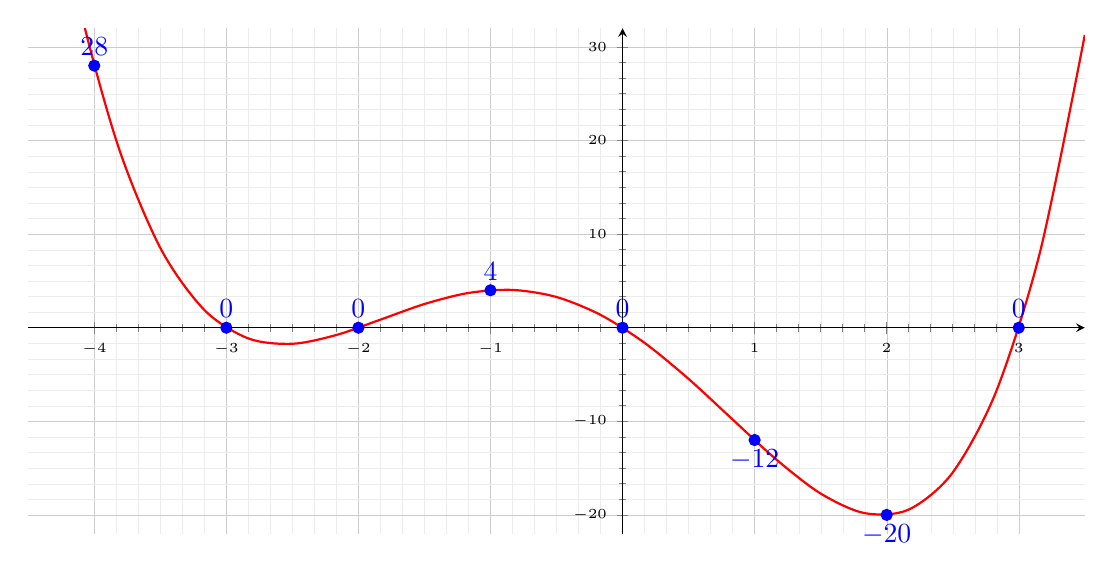
\begin{tikzpicture}
\begin{axis}[
    % Set the overall dimensions of the plot area
    height=8cm, 
    width=15cm,  
    % Set the domain and range for the axes
    xmin=-4.5, xmax=3.5,
    ymin=-22, ymax=32,
    % Manually set the tick marks
    xtick={-4,-3,-2,-1,0,1,2,3},
    ytick={-20,-10,0,10,20,30},
    % Add 5 minor lines between each major tick on both axes
    minor x tick num=5,
    minor y tick num=5,
    % This command draws both major and minor grid lines
    grid=both,
    major grid style={line width=.1pt,draw=gray!40},
    minor grid style={line width=.1pt,draw=gray!15},
    % Axis and label styling
    axis lines=middle,
    tick label style={font=\tiny},
    xlabel style={at={(current axis.right of origin)}, anchor=west},
    ylabel style={at={(current axis.above origin)}, anchor=south},
    axis line style={-stealth},
]

\addplot[domain=-4.5:3.5, smooth, thick, red] {(1/2)*(x)*(x-3)*(x+3)*(x+2)};
    
\addplot[only marks, mark=*, blue, nodes near coords]
  coordinates {
    (-4, 28)
    (-3, 0)
    (-2, 0)
    (-1, 4)
    (0, 0)
    (1, -12)
    (2, -20)
    (3, 0)
  };
\end{axis}
\end{tikzpicture}


 \end{document}